\documentclass[11pt]{article}

\usepackage{graphicx, epsfig}
\usepackage{amsmath, amssymb, latexsym}
\usepackage[english]{babel}
\usepackage{amssymb}   
%\usepackage{graphicx}
%\usepackage{float} 






% Make a larger page (shrink the margins)
%
\setlength{\textwidth}{6.7in}
\setlength{\textheight}{9.0in}
\setlength{\evensidemargin}{0.0in}
\setlength{\oddsidemargin}{0.0in}
\topmargin -0.5in
\footskip 0.5in



\title{Confirming Instrument Consistency Between Sites}
\author{Eric Davis}
\begin{document}
\maketitle
\medskip



\begin{figure}[h!]
\includegraphics[scale=0.7]{transittimes_plot.jpg}
\caption{This shows the transit time in universal hours of Jupiter over Fort Smith. Again a linear fit, as expected. Note the slope shows the transit time decreases by 4 min 23 seconds every day. A sidereal day is shorter than the calendar by 3 min 58 s. I have a feeling this discrepancy is a result of the motion of Jupiter, but I'd like to confirm.}
\end{figure}


\section{Time Profiles}
\hspace{0.5cm}

As you are probably aware, I have used the Forth Smith data to locate an object consistently that could be useful for calibration. As luck would have it, Jupiter appears to satisfy the requirement that a) Its apparent magnitude changes slightly in the time frame for the data (approximately 30 days) and b) is consistently visible for the time frame of the data in the Northern hemisphere i.e. all the ground sites I will be looking at. So far I have only looked at Fort Smith data, but there is no reason to think Jupiter will not be clearly visible from the other sites. One thing that will be need to accounted for is the seeing from the individual sights for the specific days. If I have enough data points any outliers that are a result of something weird happening in the atmosphere will be excluded for the purposes of the analysis.   



\begin{figure}[h!]
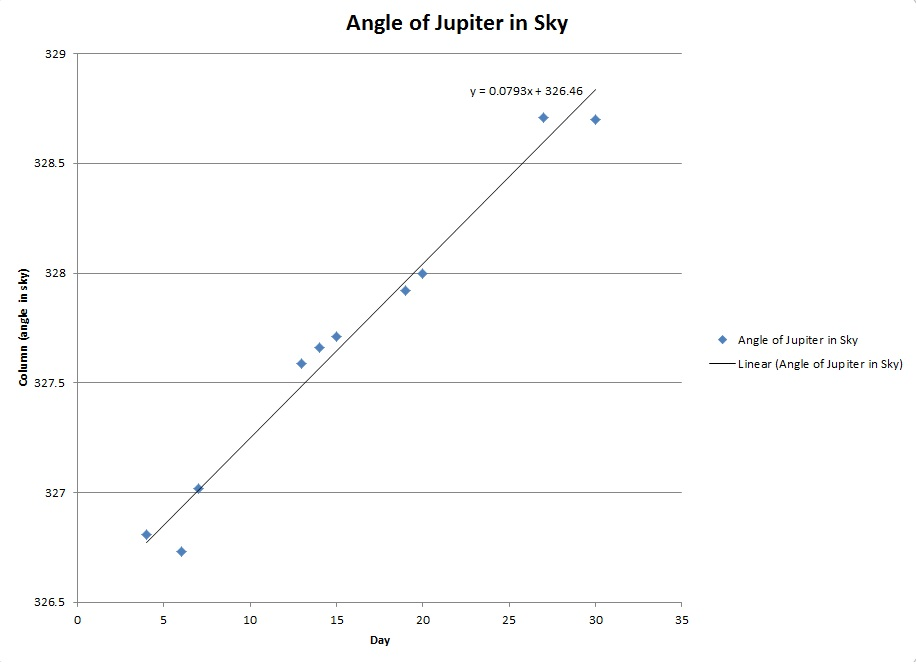
\includegraphics[scale=0.7]{jupiter_angle_vs_day.jpg}
\caption{The location (angle) of Jupiter in the sky as a function of day. It is linear as expected, but there are a couple outliers that I want to go over to see what's causing them. I highly doubt Jupiter decided to change direction on only two nights}
\end{figure}

\section{The Process}
\hspace{0.5cm}
Although I have not showed them here, I am sure you are aware I have Gaussian time and space profiles for Jupiter on 11 separate nights over 30 days. I would like to compare all of the filters from all of the sites. I should be able to in the first couple days next week to have the Gaussian data from all of the sites. Although Jupiter might not be visible on the exact same days at he various sites, I should be able to get the data from the same 30 days. I will than perform all the same analyses that I did for Fort Smith. The first thing I want to check is the FWHM for every filter from all of the sites, ideally on the same night. Then repeat this for as many nights as time allows. A similar FWHM of Jupiter for both time and space profiles for all the instruments is a very strong indication that the camera is imaging the same shape. As well, I will want to look at the total amount of photons the cameras receive from Jupiter from the different sites for each filter. This should allow for absolute calibration if we can measure the total flux received by the instruments. By comparing the Gaussian parameters of Jupiter on the various instruments should tell us if the shape of the object is the same for all the imagers. As well, by doing a similar plot as seen in Figure 2 I should be able to determine if the object is being tracked as it should for all the cameras, and whether or not the tracking is the same at the different sites. 


\section{Future Considerations}

If at all possible it would be nice to perform a similar analysis for some stars, but I'm not sure if there is enough data to be able to do that. 


\end{document}
\end{article}